
%{{第四十九回}}{第四十九回}}

\chapter{琉璃世界白雪红梅 脂粉香娃割腥啖膻}\label{part0053_split_000.htmlux5cux23calibre_pb_0}

{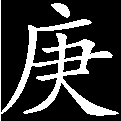
\includegraphics[width=3mm]{../Images/00004}此回系大观园集十二正钗之文。}

{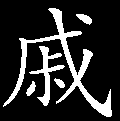
\includegraphics[width=3mm]{../Images/00005}此回原为起社,而起社却在下回。然起社之地、起社之人、起社之景、起社之题、起社之酒肴,色色皆备。真令人跃然起舞。}

话说香菱见众人正说笑,他便迎上去笑道:``你们看这一首。若使得,我便还学;若还不好,我就死了这作诗的心了。''{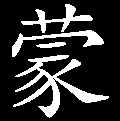
\includegraphics[width=3mm]{../Images/00006}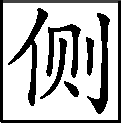
\includegraphics[width=3mm]{../Images/00011}\footnotesize \kaishu 说``死了心不学'',方是才人``语不惊人死不休''本怀!}说着,把诗递与黛玉及众人看时,只见写道是:

精华欲掩料应难,影自娟娟魄自寒。

一片砧敲千里白,半轮鸡唱五更残。

绿蓑江上秋闻笛,红袖楼头夜倚栏。

博得嫦娥应借问,缘何不使永团圆!

众人看了笑道:``这首不但好,而且新巧有意趣。可知俗语说`天下无难事,只怕有心人',社里一定请你了。''香菱听了心下不信,{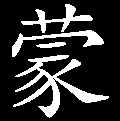
\includegraphics[width=3mm]{../Images/00006}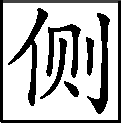
\includegraphics[width=3mm]{../Images/00011}\footnotesize \kaishu 听了不信,方是才人虚心。香菱可爱。}料着是他们瞒哄自己的话,还只管问黛玉、宝钗等。

正说之间,只见几个小丫头并老婆子忙忙的走来,都笑道:``来了好些姑娘奶奶们,我们都不认得,奶奶姑娘们快认亲去。''李纨笑道:``这是那里的话?你到底说明白了是谁的亲戚?''那婆子丫头都笑道:``奶奶的两位妹子都来了。还有一位姑娘,说是薛大姑娘的妹妹,还有一位爷,说是薛大爷的兄弟。我这会子请姨太太去呢,奶奶和姑娘们先上去罢。''说着,一迳去了。宝钗笑道:``我们薛蝌和他妹妹来了不成?''李纨也笑道:``我们婶子又上京来了不成?他们也不能凑在一处,这可是奇事。''大家纳闷,来至王夫人上房,只见乌压压一地的人。

原来邢夫人之兄嫂带了女儿岫烟进京来投邢夫人的,可巧凤姐之兄王仁也正进京,两亲家一处打帮来了。走至半路泊船时,正遇见李纨之寡婶带着两个女儿------大名李纹,次名李绮------也上京。大家叙起来又是亲戚,因此三家一路同行。后有薛蟠之从弟薛蝌,因当年父亲在京时已将胞妹薛宝琴许配都中梅翰林之子为婚,{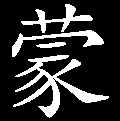
\includegraphics[width=3mm]{../Images/00006}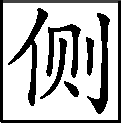
\includegraphics[width=3mm]{../Images/00011}\footnotesize \kaishu 宝琴许配梅门,于叙事内先逗一笔,后方不突{(实)}{[}然{]}。此等法脉,识者着眼。}正欲进京发嫁,闻得王仁进京,他也带了妹子随后赶来。所以今日会齐了来访投各人亲戚。

于是大家见礼叙过,贾母王夫人都欢喜非常。贾母因笑道:``怪道昨日晚上灯花爆了又爆,结了又结,{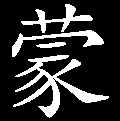
\includegraphics[width=3mm]{../Images/00006}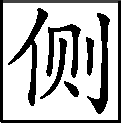
\includegraphics[width=3mm]{../Images/00011}\footnotesize \kaishu ``灯花''二语何等扯淡,何等包括有趣。着俗笔则语{(喇喇)}{[}剌剌{]}而不休矣。}原来应到今日。''一面叙些家常,一面收看带来的礼物,一面命留酒饭。凤姐儿自不必说,忙上加忙。李纨宝钗自然和婶母姊妹叙离别之情。黛玉见了,先是欢喜,{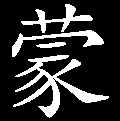
\includegraphics[width=3mm]{../Images/00006}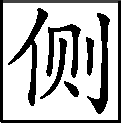
\includegraphics[width=3mm]{../Images/00011}\footnotesize \kaishu 黛玉先喜后悲,不悲非情,不喜又非情。作\ldots{}\ldots{}}次后想起众人皆有亲眷,独自己孤单,无个亲眷,不免又去垂泪。宝玉深知其情,十分劝慰了一番方罢。

然后宝玉忙忙来至怡红院中,向袭人、麝月、晴雯等笑道:``你们还不快看人去!谁知宝姐姐的亲哥哥是那个样子,他这叔伯兄弟形容举止另是一样了,倒像是宝姐姐的同胞弟兄似的。更奇在你们成日家只说宝姐姐是绝色的人物,你们如今瞧瞧他这妹子,更有大嫂嫂这两个妹子,我竟形容不出了。老天,老天,你有多少精华灵秀,生出这些人上之人来!可知我井底之蛙,成日家自说现在的这几个人是有一无二的,谁知不必远寻,就是本地风光,一个赛似一个,如今我又长了一层学问了。除了这几个,难道还有几个不成?''一面说,一面自笑自叹。袭人见他又有了魔意,便不肯去瞧。晴雯等早去瞧了一遍回来,{{(坎坎)}}{[}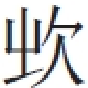
\includegraphics[width=4mm]{../images/00025}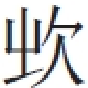
\includegraphics[width=4mm]{../images/00025}{]}笑向袭人道:``你快瞧瞧去!大太太的一个侄女儿,宝姑娘一个妹妹,大奶奶两个妹妹,倒像一把子四根水葱儿。''

一语未了,只见探春也笑着进来找宝玉,因说道:``咱们的诗社可兴旺了。''宝玉笑道:``正是呢。这是你一高兴起诗社,所以鬼使神差来了这些人。但只一件,不知他们可学过作诗不曾?''探春道:``我才都问了问他们,虽是他们自谦,看其光景,没有不会的。便是不会也没难处,你看香菱就知道了。''袭人笑道:``他们说薛大姑娘的妹妹更好,三姑娘看着怎么样?''探春道:``果然的话。据我看,连他姐姐并这些人总不及他。''袭人听了,又是诧异,又笑道:``这也奇了,还从那里再好的去呢?我倒要瞧瞧去。''探春道:``老太太一见了,喜欢的无可不可,已经逼着太太认了干女儿了。老太太要养活,才刚已经定了。''宝玉喜的忙问:``这果然的?''探春道:``我几时说过谎!''又笑道:``有了这个好孙女儿,就忘了这孙子了。''宝玉笑道:``这倒不妨,原该多疼女儿些才是正理。明儿十六,咱们可该起社了。''探春道:``林丫头刚起来了,二姐姐又病了,终是七上八下的。''宝玉道:``二姐姐又不大作诗,没有他又何妨。''探春道:``越性等几天,他们新来的混熟了,咱们邀上他们岂不好?这会子大嫂子宝姐姐心里自然没有诗兴的,况且湘云没来,颦儿刚好了,人人不合式。不如等着云丫头来了,这几个新的也熟了,颦儿也大好了,大嫂子和宝姐姐心也闲了,香菱诗也长进了,如此邀一满社岂不好?咱们两个如今且往老太太那里去听听,除宝姐姐的妹妹不算外,他一定是在咱们家住定了的。倘或那三个要不在咱们这里住,咱们央告着老太太留下他们在园子里住下,咱们岂不多添几个人,越发有趣了。''宝玉听了,喜的眉开眼笑,忙说道:``倒是你明白。{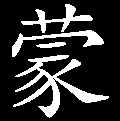
\includegraphics[width=3mm]{../Images/00006}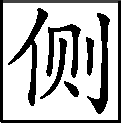
\includegraphics[width=3mm]{../Images/00011}\footnotesize \kaishu 观宝玉``到底是你''数语,胸中纯是一团活泼泼天机。}我终久是个糊涂心肠,空喜欢一会子,却想不到这上头来。''

说着,兄妹两个一齐往贾母处来。果然王夫人已认了宝琴作干女儿,贾母欢喜非常,连园中也不命住,晚上跟着贾母一处安寝。薛蝌自向薛蟠书房中住下。贾母便和邢夫人说:``你侄女儿也不必家去了,园里住几天,逛逛再去。''邢夫人兄嫂家中原艰难,这一上京,原仗的是邢夫人与他们治房舍,帮盘缠,听如此说,岂不愿意。邢夫人便将岫烟交与凤姐儿。凤姐儿筹算得园中姊妹多,性情不一,{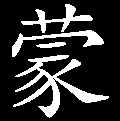
\includegraphics[width=3mm]{../Images/00006}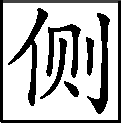
\includegraphics[width=3mm]{../Images/00011}\footnotesize \kaishu 凤姐一番筹算,总为与自己无干。奸雄每每如此。我爱之,我恶之。}且又不便另设一处,莫若送到迎春一处去,倘日后邢岫烟有些不遂意的事,纵然邢夫人知道了,与自己无干。从此后若邢岫烟家去住的日期不算,若在大观园住到一个月上,凤姐儿亦照迎春的分例送一分与岫烟。凤姐儿冷眼敁敠{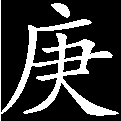
\includegraphics[width=3mm]{../Images/00004}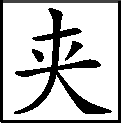
\includegraphics[width=3mm]{../Images/00012}\footnotesize \kaishu 音``颠夺'',心内忖度也。}岫烟心性为人,{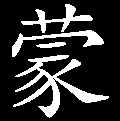
\includegraphics[width=3mm]{../Images/00006}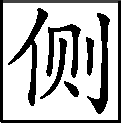
\includegraphics[width=3mm]{../Images/00011}\footnotesize \kaishu 先叙岫烟,次叙李纨,又叙李纹李绮,亦何精致可玩。}竟不像邢夫人及他的父母一样,却是温厚可疼的人。因此凤姐儿又怜他家贫命苦,比别的姊妹多疼他些,邢夫人倒不大理论了。

贾母王夫人因素喜李纨贤惠,且年轻守节,令人敬伏,今见他寡婶来了,便不肯令他外头去住。那李婶虽十分不肯,无奈贾母执意不从,只得带着李纹李绮在稻香村住下来。

当下安插既定,谁知保龄侯史鼐又迁委了外省大员,不日要带家眷去上任。{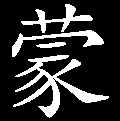
\includegraphics[width=3mm]{../Images/00006}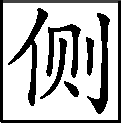
\includegraphics[width=3mm]{../Images/00011}\footnotesize \kaishu 史鼐未必左迁,但欲湘云赴社,故作此一折耳,莫被他混过。}贾母因舍不得湘云,便留下他了,接到家中,原要命凤姐儿另设一处与他住。史湘云执意不肯,只要与宝钗一处住,因此就罢了。

此时大观园中比先更热闹了多少。{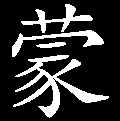
\includegraphics[width=3mm]{../Images/00006}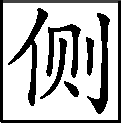
\includegraphics[width=3mm]{../Images/00011}\footnotesize \kaishu ``此时大观园''数行收拾,是大手笔。}李纨为首,馀者迎春、探春、惜春、宝钗、黛玉、湘云、李纹、李绮、宝琴、邢岫烟,再添上凤姐儿和宝玉,一共十三个。叙起年庚,除李纨年纪最长,他十二个人皆不过十五六七岁,或有这三个同年,或有那五个共岁,或有这两个同月同日,那两个同刻同时,所差者大半是时刻月分而已。连他们自己也不能\href{../Text/part0053_split_000.html\#lnkback_1_a}{\textsuperscript{①}}细细分晰,不过是``弟''``兄''
``姊''``妹''四个字随便乱叫。

如今香菱正满心满意只想作诗,又不敢十分罗唣宝钗,可巧来了个史湘云。那史湘云又是极爱说话的,那里禁得起香菱又请教他谈诗,越发高了兴,没昼没夜高谈阔论起来。宝钗因笑道:``我实在聒噪的受不得了。一个女孩儿家,只管拿着诗作正经事讲起来,叫有学问的人听了,反笑话说不守本分的。一个香菱没闹清,偏又添了你这么个话口袋子,满嘴里说的是什么:怎么是杜工部之沈郁,韦苏州之淡雅,又怎么是温八叉之绮靡,李义山之隐僻。放着两个现成的诗家不知道,提那些死人做什么!''湘云听了,忙笑问道:``是那两个?好姐姐,你告诉我。''宝钗笑道:``呆香菱之心苦,疯湘云之话多。''湘云香菱听了,都笑起来。

正说着,只见宝琴来了,披着一领斗篷,金翠辉煌,不知何物。宝钗忙问:``这是那里的?''宝琴笑道:``因下雪珠儿,老太太找了这一件给我的。''香菱上来瞧道:``怪道这么好看,原来是孔雀毛织的。''湘云道:``那里是孔雀毛,就是野鸭子头上的毛作的。可见老太太疼你了,这样疼宝玉,也没给他穿。''宝钗道:``真俗语说`各人有缘法'。他也再想不到他这会子来,既来了,又有老太太这么疼他。''湘云道:``你除了在老太太跟前,就在园里来,这两处只管顽笑吃喝。到了太太屋里,若太太在屋里,只管和太太说笑,多坐一回无妨;若太太不在屋里,你别进去,那屋里人多心坏,都是要害咱们的。''说的宝钗、宝琴、香菱、莺儿等都笑了。宝钗笑道:``说你没心,却又有心;虽然有心,到底嘴太直了。我们这琴儿就有些像你。你天天说要我作亲姐姐,我今儿竟叫你认他作亲妹妹罢了。''湘云又瞅了宝琴半日,笑道:``这一件衣裳也只配他穿,别人穿了,实在不配。''正说着,只见琥珀走来笑道:``老太太说了,叫宝姑娘别管紧了琴姑娘。他还小呢,让他爱怎么样就怎么样。要什么东西只管要去,别多心。''宝钗忙起身答应了,又推宝琴笑道:``你也不知是那里来的福气!你倒去罢,仔细我们委曲着你。我就不信我那些儿不如你。''

说话之间,宝玉、黛玉都进来了,宝钗犹自嘲笑。湘云因笑道:``宝姐姐,你这话虽是顽话,恰有人真心是这样想呢。''琥珀笑道:``真心恼的再没别人,就只是他。''口里说,手指着宝玉。宝钗湘云都笑道:``他倒不是这样人。''琥珀又笑道:``不是他,就是他。''说着又指着黛玉。湘云便不则声。{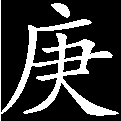
\includegraphics[width=3mm]{../Images/00004}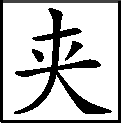
\includegraphics[width=3mm]{../Images/00012}\footnotesize \kaishu 是不知道黛玉病中相谈赠燕窝之事也。脂砚。}宝钗忙笑道:``更不是了。我的妹妹和他的妹妹一样。他喜欢的比我还疼呢,那里还恼?你信云儿混说。他的那嘴有什么实据。''宝玉素习深知黛玉有些小性儿,且尚不知近日黛玉和宝钗之事,正恐贾母疼宝琴他心中不自在,今见湘云如此说了,宝钗又如此答,再审度黛玉声色亦不似往时,果然与宝钗之说相符,心中闷闷不解。因想:``他两个素日不是这样的好,今看来竟更比他人好十倍。''一时林黛玉又赶着宝琴叫妹妹,并不提名道姓,直是亲姊妹一般。那宝琴年轻心热,{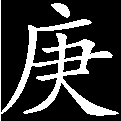
\includegraphics[width=3mm]{../Images/00004}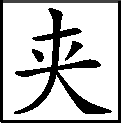
\includegraphics[width=3mm]{../Images/00012}\footnotesize \kaishu 四字道尽,不犯宝钗。脂砚斋评。}且本性聪敏,自幼读书识字,{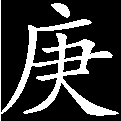
\includegraphics[width=3mm]{../Images/00004}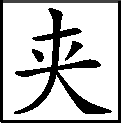
\includegraphics[width=3mm]{../Images/00012}\footnotesize \kaishu 我批此书竟得一秘诀,以告诸公:凡野史中所云``才貌双全佳人''者,细细通审之,只得一个粗知笔墨之女子耳。此书凡云``知书识字''者,便是上等才女,不信时只看他通部行为及诗词、诙谐皆可知。妙在此书从不肯自下评注,云此人系何等人,只借书中人闲评一二语,故不得有未密之缝被看书者指出,真狡猾之笔耳。}今在贾府住了两日,大概人物已知。又见诸姊妹都不是那轻薄脂粉,且又和姐姐皆和契,故也不肯怠慢,其中又见林黛玉是个出类拔萃的,便更与黛玉亲敬异常。宝玉看着只是暗暗的纳罕。

一时宝钗姊妹往薛姨妈房内去后,湘云往贾母处来,林黛玉回房歇着。宝玉便找了黛玉来,笑道:``我虽看了《西厢记》,也曾有明白的几句,说了取笑,你曾恼过。如今想来,竟有一句不解,我念出来你讲讲我听。''黛玉听了,便知有文章,因笑道:``你念出来我听听。''宝玉笑道:``那《闹简》上有一句说得最好,`是几时孟光接了梁鸿案?'这句最妙。`孟光接了梁鸿案'这七个字,不过是现成的典,难为他这`是几时'三个虚字问的有趣。是几时接了?你说说我听听。''黛玉听了,禁不住也笑起来,因笑道:``这原问的好。他也问的好,你也问的好。''宝玉道:``先时你只疑我,如今你也没的说,我反落了单。''黛玉笑道:``谁知他竟真是个好人,我素日只当他藏奸。''因把说错了酒令起,连送燕窝病中所谈之事,细细告诉了宝玉。宝玉方知缘故,因笑道:``我说呢,正纳闷`是几时孟光接了梁鸿案',原来是从`小孩儿家口没遮拦'就接了案了。''黛玉因又说起宝琴来,想起自己没有姊妹,不免又哭了。宝玉忙劝道:``你又自寻烦恼了。你瞧瞧,今年比旧年越发瘦了,你还不保养。每天好好的,你必是自寻烦恼,哭一会子,才算完了这一天的事。''黛玉拭泪道:``近来我只觉心酸,眼泪却像比旧年少了些的。心里只管酸痛,眼泪却不多。''宝玉道:``这是你哭惯了心里疑的,岂有眼泪会少的!''

正说着,只见他屋里的小丫头子送了猩猩毡斗篷来,又说:``大奶奶才打发人来说,下了雪,要商议明日请人作诗呢。''一语未了,只见李纨的丫头走来请黛玉。宝玉便邀着黛玉同往稻香村来。黛玉换上掐金挖云红香羊皮小靴,罩了一件大红羽纱面白狐狸里的鹤氅,束一条青金闪绿双环四合如意绦,头上罩了雪帽。二人一齐踏雪行来。只见众姊妹都在那边,都是一色大红猩猩毡与羽毛缎斗篷,独李纨穿一件青哆啰呢对襟褂子,薛宝钗穿一件莲青斗纹锦上添花洋线番羓丝的鹤氅;邢岫烟仍是家常旧衣,并无避雪之衣。一时史湘云来了,穿着贾母与他的一件貂鼠脑袋面子大毛黑灰鼠里子里外发烧大褂子,头上戴着一顶挖云鹅黄片金里大红猩猩毡昭君套,又围着大貂鼠风领。黛玉先笑道:``你们瞧瞧,孙行者来了。他一般的也拿着雪褂子,故意装出个小骚达子来。''湘云笑道:``你们瞧我里头打扮的。''一面说,一面脱了褂子。只见他里头穿着一件半新的靠色三镶领袖秋香色盘金五色绣龙窄褃小袖掩衿银鼠短袄,里面短短的一件水红妆缎狐肷褶子,腰里紧紧束着一条蝴蝶结子长穗五色宫绦,脚下也穿着麀皮小靴,越显的蜂腰猿背,鹤势螂形。{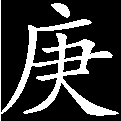
\includegraphics[width=3mm]{../Images/00004}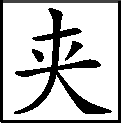
\includegraphics[width=3mm]{../Images/00012}\footnotesize \kaishu 近之拳谱中有``坐马势'',便似螂之蹲立。昔人爱轻捷便俏,闲取一螂,观其仰颈叠胸之势。今四字无出处,却写尽矣。脂砚斋评。}众人都笑道:``偏他只爱打扮成个小子的样儿,原比他打扮女儿更俏丽了些。''湘云道:``快商议作诗!我听听是谁的东家?''李纨道:``我的主意。想来昨儿的正日已过了,再等正日又太远,可巧又下雪,不如大家凑个社,又替他们接风,又可以作诗。你们意思怎么样?''宝玉先道:``这话很是。只是今日晚了,若到明儿,晴了又无趣。''众人看道:``这雪未必晴,纵晴了,这一夜下的也够赏了。''李纨道:``我这里虽好,又不如芦雪广好。我已经打发人笼地炕去了,咱们大家拥炉作诗。老太太想来未必高兴,况且咱们小顽意儿,单给凤丫头个信儿就是了。你们每人一两银子就够了,送到我这里来。''指着香菱、宝琴、李纹、李绮、岫烟,``五个不算外,咱们里头二丫头病了不算,四丫头告了假也不算,你们四分子送了来,我包总五六两银子也尽够了。''宝钗等一齐应诺。因又拟题限韵,李纨笑道:``我心里自己定了,等到了明日临期,横竖知道。''说毕,大家又闲话了一回,方往贾母处来。本日无话。

到了次日一早,宝玉因心里记挂着这事,一夜没好生得睡,天亮了就爬起来。掀开帐子一看,虽门窗尚掩,只见窗上光辉夺目,心内早踌躇起来,埋怨定是晴了,日光已出。一面忙起来揭起窗屉,从玻璃窗内往外一看,原来不是日光,竟是一夜大雪,下将有一尺多厚,天上仍是搓绵扯絮一般。宝玉此时欢喜非常,忙唤人起来,盥漱已毕,只穿一件茄色哆啰呢狐皮袄子,罩一件海龙皮小小鹰膀褂,束了腰,披了玉针蓑,戴上金藤笠,登上沙棠屐,忙忙的往芦雪广来。出了院门,四顾一望,并无二色,远远的是青松翠竹,自己却如装在玻璃盒内一般。于是走至山坡之下,顺着山脚刚转过去,已闻得一股寒香拂鼻。回头一看,恰是妙玉门前栊翠庵中有十数株红梅如胭脂一般,映着雪色,分外显得精神,好不有趣!宝玉便立住,细细的赏玩一回方走。只见蜂腰板桥上一个人打着伞走来,是李纨打发了请凤姐儿去的人。

宝玉来至芦雪广,只见丫鬟婆子正在那里扫雪开径。原来这芦雪广盖在傍山临水河滩之上,一带几间,茅檐土壁,槿篱竹牖,推窗便可垂钓,四面都是芦苇掩覆,一条去径逶迤穿芦度苇过去,便是藕香榭的竹桥了。众丫鬟婆子见他披蓑戴笠而来,都笑道:``我们才说正少一个渔翁,如今都全了。姑娘们吃了饭才来呢,你也太性急了。''宝玉听了,只得回来。刚至沁芳亭,见探春正从秋爽斋来,围着大红猩猩毡斗篷,戴着观音兜,扶着小丫头,后面一个妇人打着青绸油伞。宝玉知他往贾母处去,便立在亭边,等他来到,二人一同出园前去。宝琴正在里间房内梳洗更衣。

一时众姊妹来齐,宝玉只嚷饿了,连连催饭。好容易等摆上来,头一样菜便是牛乳蒸羊羔。贾母便说:``这是我们有年纪的人的药,没见天日的东西,可惜你们小孩子们吃不得。今儿另外有新鲜鹿肉,你们等着吃。''众人答应了。宝玉却等不得,只拿茶泡了一碗饭,就着野鸡瓜齑忙忙的咽完了。贾母道:``我知道你们今儿又有事情,连饭也不顾吃了。''便叫``留着鹿肉与他晚上吃'',凤姐忙说``还有呢'',方才罢了。史湘云便悄和宝玉计较道:``有新鲜鹿肉,不如咱们要一块,自己拿了园里弄着,又顽又吃。''宝玉听了,巴不得一声儿,便真和凤姐要了一块,命婆子送入园去。

一时大家散后,进园齐往芦雪广来,听李纨出题限韵,独不见湘云宝玉二人。黛玉道:``他两个再到不了一处,若到一处,生出多少故事来。这会子一定算计那块鹿肉去了。''{{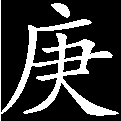
\includegraphics[width=3mm]{../Images/00004}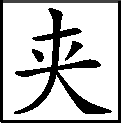
\includegraphics[width=3mm]{../Images/00012}\footnotesize \kaishu 联诗极雅之事,偏于雅前写出小儿啖膻茹血极腌}臜{的事来,为``锦心绣口''作配。}}正说着,只见李婶也走来看热闹,因问李纨道:``怎么一个带玉的哥儿和那一个挂金麒麟的姐儿,那样干净清秀,又不少吃的,他两个在那里商议着要吃生肉呢,说的有来有去的。我只不信肉也生吃得的。''众人听了,都笑道:``了不得,快拿了他两个来。''黛玉笑道:``这可是云丫头闹的,我的卦再不错。''

李纨等忙出来找着他两个说道:``你们两个要吃生的,我送你们到老太太那里吃去。那怕吃一只生鹿,撑病了不与我相干。这么大雪,怪冷的,替我作祸呢。''宝玉笑道:``没有的事,我们烧着吃呢。''李纨道:``这还罢了。''只见老婆子们拿了铁炉、铁叉、铁丝蒙来,李纨道:``仔细割了手,不许哭!''说着,同探春进去了。

凤姐打发了平儿来回复不能来,为发放年例正忙。湘云见了平儿,那里肯放。平儿也是个好顽的,素日跟着凤姐儿无所不至,见如此有趣,乐得顽笑,因而褪去手上的镯子,三个围着火炉儿,便要先烧三块吃。那边宝钗黛玉平素看惯了,不以为异,宝琴等及李婶深为罕事。探春与李纨等已议定了题韵。探春笑道:``你闻闻,香气这里都闻见了,我也吃去。''说着,也找了他们来。李纨也随来说:``客已齐了,你们还吃不够?''湘云一面吃,一面说道:``我吃这个方爱吃酒,吃了酒才有诗。若不是这鹿肉,今儿断不能作诗。''说着,只见宝琴披着凫靥裘站在那里笑。湘云笑道:``傻子,过来尝尝。''宝琴笑说:``怪脏的。''宝钗道:``你尝尝去,好吃的。你林姐姐弱,吃了不消化,不然他也爱吃。''宝琴听了,便过去吃了一块,果然好吃,便也吃起来。一时凤姐儿打发小丫头来叫平儿。平儿说:``史姑娘拉着我呢,你先走罢。''小丫头去了。一时只见凤姐也披了斗篷走来,笑道:``吃这样好东西,也不告诉我!''说着也凑着一处吃起来。黛玉笑道:``那里找这一群花子去!罢了,罢了,今日芦雪广遭劫,生生被云丫头作践了。我为芦雪广一大哭!''{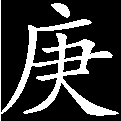
\includegraphics[width=3mm]{../Images/00004}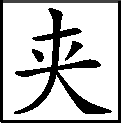
\includegraphics[width=3mm]{../Images/00012}\footnotesize \kaishu 大约此话不独黛玉,观书者亦如此。}湘云冷笑道:``你知道什么!`是真名士自风流',你们都是假清高,最可厌的。我们这会子腥膻大吃大嚼,回来却是锦心绣口。''宝钗笑道:``你回来若作的不好了,把那肉掏了出来,就把这雪压的芦苇子揌上些,以完此劫。''

说着,吃毕,洗漱了一回。平儿带镯子时却少了一个,左右前后乱找了一番,踪迹全无。众人都诧异。凤姐儿笑道:``我知道这镯子的去向。你们只管作诗去,我们也不用找,只管前头去,不出三日包管就有了。''说着又问:``你们今儿做什么诗?老太太说了,离年又近了,正月里还该作些灯谜儿大家顽笑。''众人听了,都笑道:``可是倒忘了。如今赶着作几个好的,预备正月里顽。''说着,一齐来至地炕屋内,只见杯盘果菜俱已摆齐,墙上已贴出诗题、韵脚、格式来了。宝玉湘云二人忙看时,只见题目是``即景联句,五言排律一首,限`二萧'韵''。后面尚未列次序。李纨道:``我不大会作诗,我只起三句罢,然后谁先得了谁先联。''宝钗道:``到底分个次序。''要知端的,且听下回分解。

{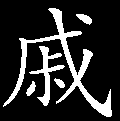
\includegraphics[width=3mm]{../Images/00005}总评:此文线索在斗篷。宝琴翠羽斗篷,贾母所赐,言其亲也;宝玉红猩猩毡斗篷,为后雪披一衬也;黛玉白狐皮斗篷,明其弱也;李宫裁斗篷是哆}啰{呢,昭其质也;宝钗斗篷是莲青斗纹锦,致其文也;贾母是大斗篷,尊之词也;凤姐是披着斗篷,恰似掌家人也;湘云有斗篷不穿,着其异样行动也;岫烟无斗篷,叙其穷也。只一斗篷,写得前后照耀生色。}

{一片含梅咀雪文字,偏从雉肉、鹿肉、鹌鹑肉上以渲染之,点成异样笔墨,较之雪吟、雪赋诸作,更觉幽秀。}

{\href{../Text/part0053_split_000.html\#navto_1_a}{①}此处诸本多``记清谁长谁幼,一并贾母、王夫人及家中婆子、丫头也不能''共23字,或谓系底本因``也不能''三字重出而脱文。按:当事人``自己都不能记清'',别人当然更不能,加这句纯属蛇足。底本应非脱文。}
